\begin{bibunit}
\thispagestyle{plain}

% Add missing command definitions from original paper
\newcommand{\commentcolour}[3]{\textcolor{#3}{[\textbf{#1:} #2]}}
\newcommand{\commentVV}[1]{\commentcolour{VV}{#1}{orange}}
\newcommand{\VV}[1]{\textcolor{orange}{#1}}
\newcommand{\soutVV}[1]{\VV{\sout{#1}}}
\newcommand{\corrVV}[2]{\sout{#1} \VV{#2}}
\newcommand{\N}{{\mathbb N}}
\newcommand{\NN}{\mathcal N}
\newcommand{\etal}{\it et al. \normalfont}


\section*{Abstract}

This paper introduces an innovative multiactor framework that harnesses the potential of LLMs to augment the functionalities of ICS. By integrating conversational AI technologies, this framework significantly improves human-machine interactions, enabling sophisticated analysis and visualization of intricate data sets.  The core of the system comprises specialized LLM actors that interact through a LangGraph-based multi-actor framework, addressing various aspects of IEC 61499 control systems including PLC code analysis, SQL query execution, and data visualization. This integration enables operators to interact with the control system using natural language, significantly reducing technical barriers and enhancing the accessibility and usability of complex industrial systems. 
    
\section{Introduction}

IEC 61499 \cite{iec61499part12012} is an international standard for distributed control systems that defines a model for structuring and developing industrial automation systems. It extends the capabilities of its predecessor, IEC 61131-3 \cite{tiegelkamp2010iec}, by emphasizing modularity, interoperability, and portability. The primary advantage of IEC 61499 is its ability to facilitate the design and deployment of flexible and reusable control systems, which can adapt to changing process requirements without extensive reprogramming. This standard supports event-driven control activities, enabling more responsive and efficient systems, particularly suitable for complex, distributed industrial environments.

The implementation of IEC 61499 \cite{vyatkin2009iec} improves the development of industrial control systems (ICS) by providing a framework that allows the seamless integration of various components and subsystems. It enables the creation of robust and scalable control solutions that can operate across different hardware and software platforms. By fostering a modular design approach, IEC 61499 reduces development time and costs while improving system reliability and maintainability. 

ICS face significant challenges in data retrieval and analysis \cite{cho2023dynamic}. The vast amount of data generated and recorded in databases is often complex and cumbersome to analyze due to its sheer volume and variety \cite{stojanovic2020challenges}. Traditional methods, which frequently rely on SQL queries for data retrieval, can be inefficient and time-consuming, requiring specialized skills to formulate and execute. This complexity hinders the ability to quickly extract actionable insights from the data, which is critical to timely decision-making and operational adjustments.

In this context, LLMs \cite{chang2024survey} offer transformative potential to advance information retrieval and data analysis within industrial settings. By interfacing with databases using the conversational language, LLMs can streamline the data querying and analyzing process, making it more accessible and less reliant on specialized query languages \cite{rajkumar2022evaluating}. 

In this paper, we present a multi-actor system designed for intelligent data analysis and visualization utilizing LLMs. The system comprises distinct actors, each specialized in particular tasks. These LLM actors are integrated to develop capabilities for responding to inquiries concerning the control system based on its Programmable Logic Controller (PLC) code, SQL queries, and the graphical representation of recorded values. This integration facilitates the accessibility of advanced data analytics through natural language, improving the interpretability and usability of complex data sets within industrial environments.

\begin{figure*}
    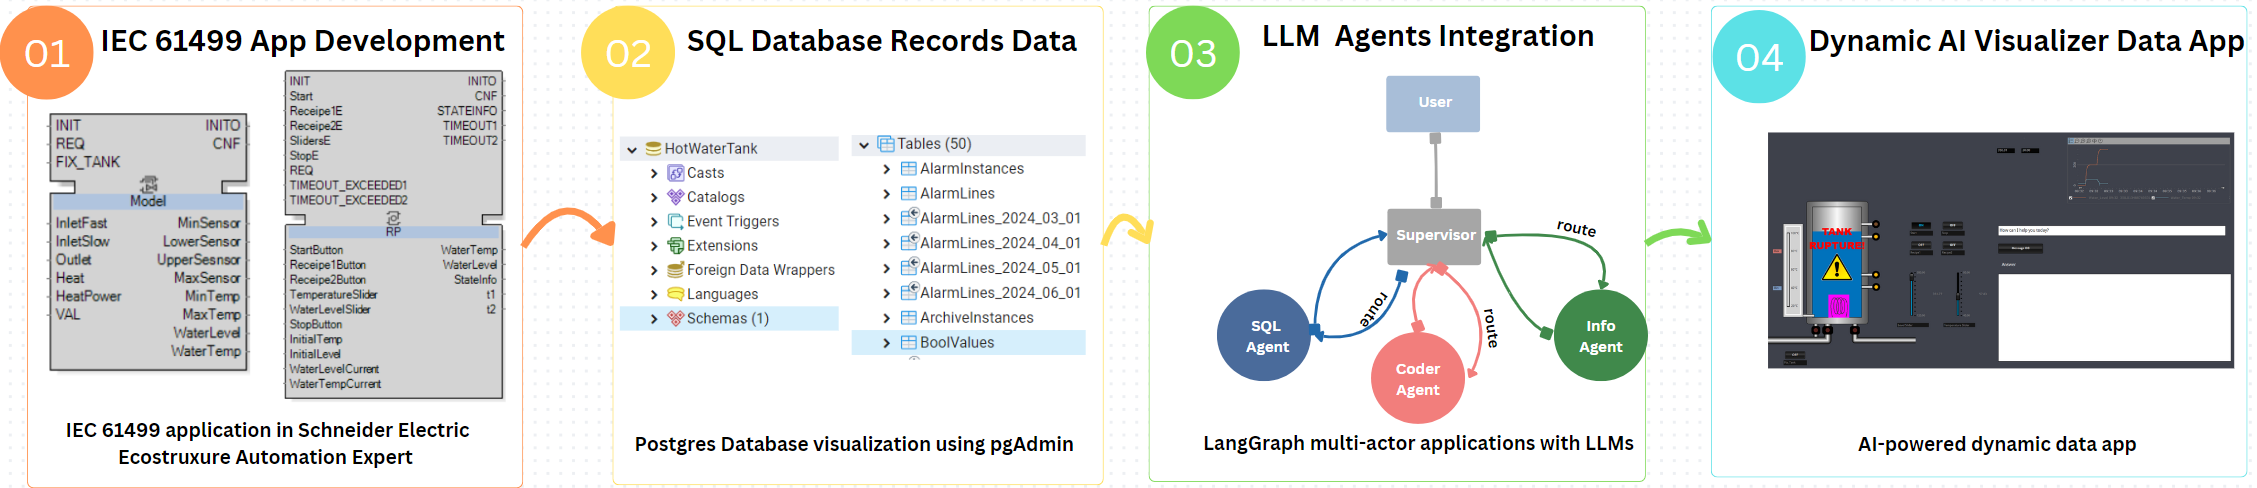
\includegraphics[width=1\textwidth]{MX_Papers/Paper12/images/workflow.PNG}
    \caption{Workflow for developing an intelligent multi-actor application with LLMs for data analysis and visualization of IEC 61499-based control systems}
    \label{fig:workflow_diagram}
\end{figure*}

\section{LLM in Industrial Control Systems}
\label{sec: LLM in ICS}

An LLM \cite{wang2024survey} is a type of artificial intelligence algorithm trained on large amounts of text data to understand and generate human-like text. These models, built on architectures such as the transformer, have the ability to process and predict sequences of words, allowing them to perform a variety of linguistic tasks. LLMs excel in areas such as natural language understanding (NLU) and natural language generation (NLG), making them highly effective for tasks that involve language translation, summarization, question answering, etc. \cite{wei2022emergent}. 

Among the most notable LLMs are OpenAI's GPT (Generative Pre-trained Transformer) series \cite{openai2023introducinggpts}, Google's BERT (Bidirectional Encoder Representations from Transformers) \cite{google2018bert}, and Meta's Llama 3 \cite{metallama3}. Each of these models has set benchmarks in the field of natural language processing by delivering state-of-the-art performance across various linguistic tasks. GPT-3, for instance, is renowned for its ability to generate coherent and contextually relevant text over extended passages, while BERT specializes in understanding the context of words in sentences, which enhances its effectiveness in understanding search queries and information retrieval.

The integration of LLMs into ICS significantly enhances Human-Machine Interfaces (HMIs) \cite{kiangala2024experimental}, making them more intuitive and accessible through conversational AI. Operators can interact with machines using natural language to perform tasks such as querying system status, issuing commands, or troubleshooting, which reduces technical barriers and improves user experience \cite{kernan2024knowledge}. LLMs also revolutionize documentation and reporting by automating the creation of detailed operational records and incident reports, improving the accuracy and timeliness of critical data for compliance and operational reviews \cite{hays2024employing}. These models offer predictive maintenance capabilities by analyzing historical and real-time data to predict equipment failures, thus minimizing downtime and extending the useful life of the equipment \cite{myohanen2023improving}. In multinational industrial operations, LLMs enable real-time translation of language, enhancing communication and collaboration between diverse teams \cite{mangaonkar2024enhancing}. However, their deployment must address challenges related to security, data privacy, reliability, and cost to ensure that they do not compromise the operational integrity or safety of industrial systems \cite{yao2024survey}. In this paper, we enhance the Human-Machine Interface (HMI) by incorporating conversational AI, enabling it to interact with machines using natural language. This advanced interface allows for tasks such as querying system statuses, analyzing operational records, and visualizing data. 

\section{Background}
\label{sec:background}


\subsection{Langchain}

LangChain \cite{langchainai2023github} is an advanced software library designed to enhance the functionality of LLMs by facilitating the integration of external knowledge and reasoning capabilities. This framework supports the seamless combination of natural language processing tasks with data retrieval, offering a structured approach to managing workflows that incorporate external APIs, databases, and custom logic. Using LangChain, developers can extend the utility of LLMs beyond mere text generation, allowing these models to act as more comprehensive decision-making and problem solving tools within diverse applications ranging from automated customer support to dynamic content generation and complex data analysis.

\subsection{LangGraph}

LangGraph \cite{langchainailanggraph2023} is an innovative framework designed to increase the capabilities of LLMs by integrating them with graph-based data structures. This integration allows LLMs to leverage structured information in the form of graphs, enhancing their ability to understand relationships and dependencies between various entities and concepts. By utilizing LangGraph, LLMs can access and manipulate knowledge graphs, which store information in nodes and edges representing entities and their interconnections, respectively. This structured approach enables more precise and context-sensitive responses, improves reasoning on connected data, and facilitates complex decision-making processes.



\section{Workflow Description}

The workflow diagram for developing an intelligent multi-actor application with LLMs for data analysis and visualization of IEC 61499-based control systems is presented in Figure \ref{fig:workflow_diagram}. The process is divided into four stages: Initially, an IEC 61499 application is constructed to manage real-time data from various control system components such as sensors and actuators, stored in an SQL database. Next, a multi-actor application using LangGraph and LLMs is developed for enhanced data analysis and visualization. Finally, this system is integrated into a human-machine interface (HMI), employing AI functionalities from the multi-agent LLM system to enable efficient user interaction and streamline data analysis across the industrial control system. This framework offers a robust model for optimizing information retrieval and analysis within any industrial setting.


\section{Multi-Actor LLM Application for IEC 61499-Based Control System}
\label{sec:methodology}

LLMs have recently received increased recognition across various sectors due to their broad applicability. These models can be effectively integrated into ICS to enhance automation, monitoring, and maintenance processes. This paper discusses the development of an application powered by LLMs, tailored for IEC 61499. The predominant framework utilized to build applications with LLM is LangChain, which facilitates development, productionization, and deployment. In this research, LLM actors are developed to perform specific tasks, and these actors are configured to collaboratively respond to user queries. The design of this system is supported by LangGraph, which constructs robust and stateful multiactor applications with LLMs by representing steps as edges and nodes within a graph structure. Initially, the paper outlines the development of agents, followed by a case study that illustrates the utilization of these agents in a control system context. Although three distinct agents are developed in this study, the framework allows expansion to include additional agents as required to meet specific needs.

\subsection{Integrating IEC 61499 XML Data into LLMs Using Retrieval Augmented Generation}

The Info Agent, designed for data retrieval and analysis of PLC code, is depicted in Figure \ref{fig:Architecture} (B1). This application excels in responding to queries based on specific source information through a method known as Retrieval Augmented Generation (RAG). RAG is a technique that enhances the knowledge base of LLMs with additional data. Although LLMs can process information on a wide range of topics, their knowledge is inherently constrained to the public data available up to the time they were trained. To develop AI applications that can deliberate on private data or information introduced after a model's training cut-off, it is essential to augment the model's knowledge with pertinent information. This augmentation process, termed Retrieval Augmented Generation, involves curating the relevant information and incorporating it into the model's prompt to refine its responses.

In the specific context of ICS, the use of IEC 61499 XML files as supplementary data for LLMs enhances their understanding of the system intricacies. Once an application based on the IEC 61499 standard is developed, these XML files can be fed into the system, enabling the LLM to provide detailed insights about the system, devices, CAT applications, composite and basic function blocks (FBs) , HMI, adapters, and more. A typical RAG application involves two main components: Indexing and Retrieval and Generation. Indexing is an offline process that involves loading the data via DocumentLoaders, splitting large documents into manageable chunks using text splitters for easier indexing and model feeding, and storing these chunks in a VectorStore with an Embeddings model for later retrieval. The Retrieval and Generation phase operates in real-time, where upon receiving a user query, relevant document splits are retrieved using a Retriever. Subsequently, a ChatModel or LLM generates a response by crafting a prompt that includes both the question and the retrieved data, thereby producing a contextually accurate answer.


\subsection{Enabling Iterative Query Techniques  for Dynamic Data Interaction in SQL Databases} 

The SQL Agent is shown in the Figure \ref{fig:Architecture} (B2) offers a sophisticated method for constructing a Query \& Answer chain over a SQL database, allowing users to pose questions about the data and receive answers in natural language. A key feature distinguishing the SQL agent from simpler implementations is its capability to iteratively query the database multiple times as required to fully address the posed question. LangChain's SQL Agent provides a more dynamic interaction with SQL databases compared to standard query chains, offering several significant advantages. It enables the agent to answer queries not only based on the content within the databases but also using the databases’ schema, such as descriptions of specific tables. The agent is equipped to handle errors effectively by catching tracebacks from failed query executions and regenerating the queries correctly. 

Real-time operational data from an IEC 61499 application, such as sensor readings, actuator statuses, button interactions, and ECC state information, is recorded in a PostgreSQL database. The SQL Agent leverages this database to retrieve this information through natural language queries. The process within a SQL chain or agent begins by converting user input into a SQL query. Once formulated, the query is executed against the PostgreSQL database, which represents a critical juncture in the creation of a SQL chain due to the potential risks associated with automated query execution. It is crucial to carefully evaluate the security implications of running automated queries and to restrict database connection permissions as much as possible. To mitigate these risks, it may be advisable to incorporate a human approval step before executing queries. Following the safe execution of the query, the final step involves synthesizing the original question with the SQL query result. This is achieved by re-submitting the question along with the result back to the LLM, thereby generating the final answer.

To enhance the performance of agents, the implementation of a custom prompt embedded with IEC 61499 specific knowledge is proposed. This initiative involves the development of a few-shot prompt with an example selector, designed to dynamically construct the prompt based on user inputs. Such a configuration will enable the model to formulate more accurate queries by incorporating relevant questions tied to the existing database, thereby improving the precision and relevance of the generated responses.

To ensure the accurate filtering of columns containing proper nouns, such as variable names utilized within IEC 61499 applications, a  verification of spelling is required. To facilitate this, a vector store containing all distinct proper nouns from the database will be created. This will allow the agent to consult the vector store whenever a proper noun is mentioned in a user query, thereby ascertaining the correct spelling of the term. This process ensures that the agent accurately identifies the entity referenced by the user, which is critical for constructing the appropriate query.

\begin{lstlisting} 
variables = query_as_list(db, "SELECT \"Path\" FROM public.\"ArchiveInstances\";")
vector_db = FAISS.from_texts(variables , OpenAIEmbeddings())
retriever = vector_db.as_retriever(search_kwargs={"k": 1})
description = """ Use to look up values to filter on. Input is an approximate spelling of the proper noun, output is valid proper nouns. Use the noun most similar to the search."""
retriever_noun_tool = create_retriever_tool(
    retriever,
    name="search_nouns",
    description=description,)
\end{lstlisting}

The provided code snippet outlines a sequence of operations designed to facilitate the retrieval of proper nouns from a database, ensuring accurate query formulation based on user input. Initially, it extracts a list of 'Path' values from the 'ArchiveInstances' table in a PostgreSQL database, which are then transformed into a vectorized format using the FAISS library and OpenAI embeddings, enabling efficient similarity searches. Finally, a retrieval tool named 'search\_nouns' is created with a retriever object, designed to find and suggest the most similar valid proper nouns based on approximate user inputs, enhancing the accuracy of data filtering and selection.


\begin{figure*}
    \centering
    % First figure
    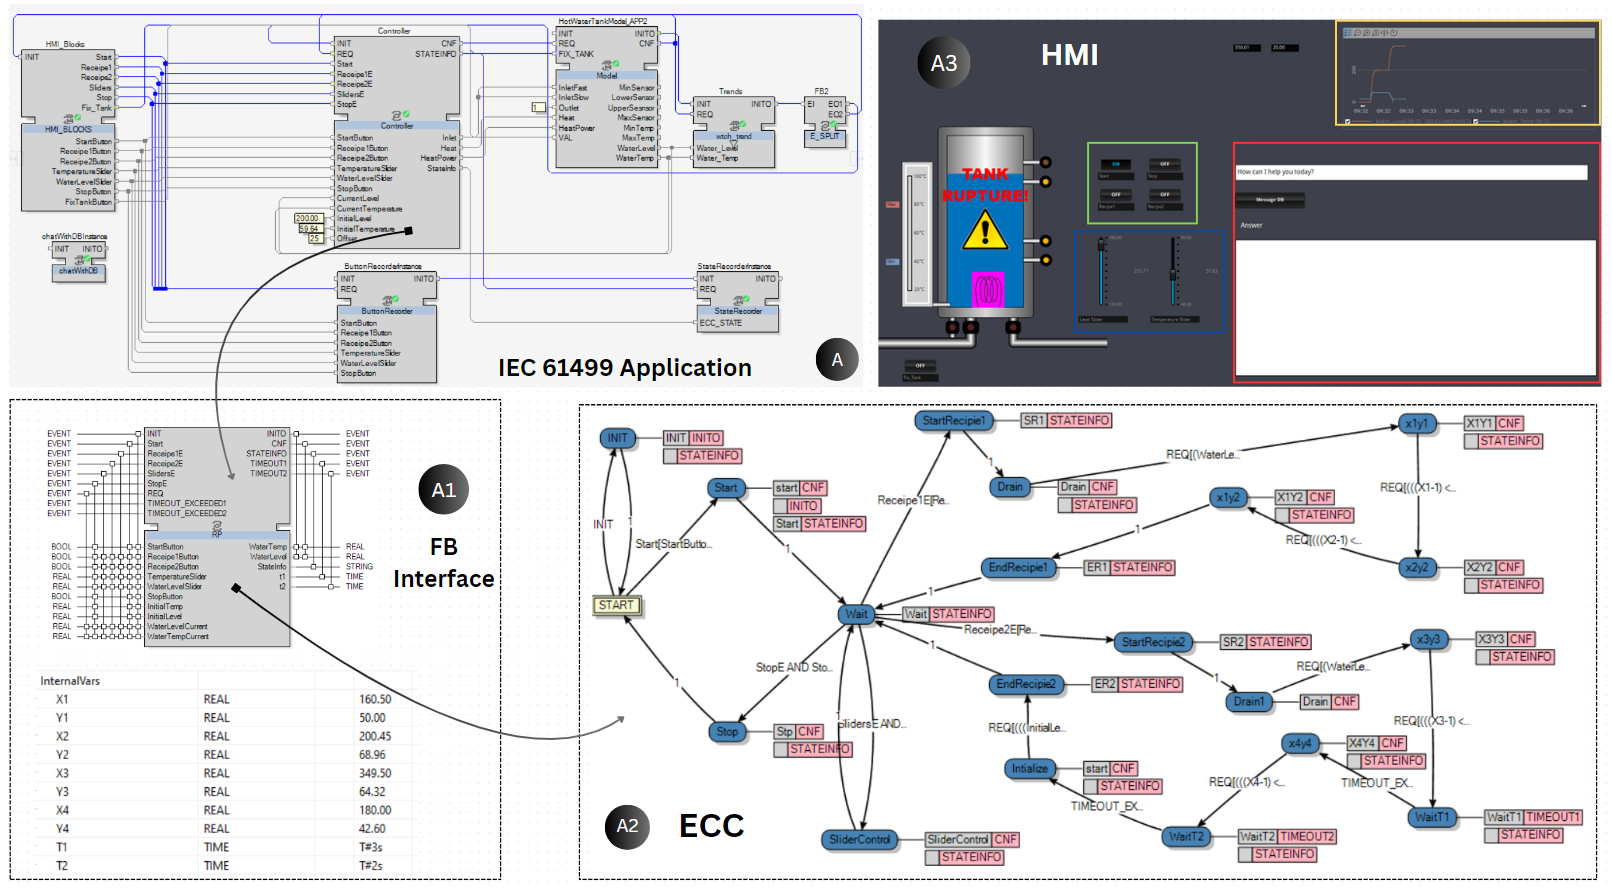
\includegraphics[width=.8\textwidth]{MX_Papers/Paper12/images/IEC61499App.PNG}
    % Second figure
    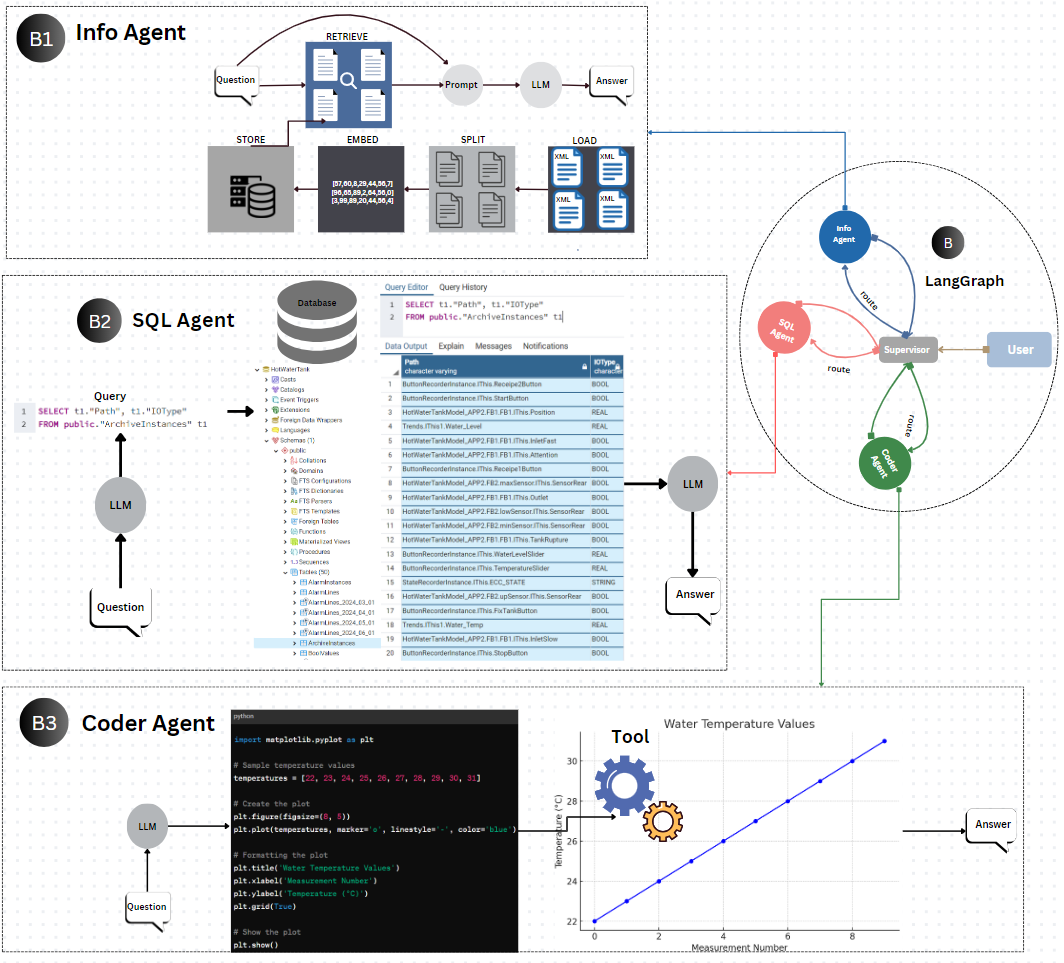
\includegraphics[width=.8\textwidth]{MX_Papers/Paper12/images/LangGraph.PNG}
    \caption{Architecture for building stateful, multi-actor applications with LLMs.}
    \label{fig:Architecture}
\end{figure*}


\subsection{Enhancing LLM Functionality with Tool Integration for Dynamic Data Visualization}

In this experiment, the objective is to utilize values extracted from a database to plot a graph, demonstrating an advanced application of Chains and Agents that can invoke Tools—ranging from APIs and functions to databases is shown in the figure \ref{fig:Architecture} (B3). Tools enhance the capabilities of a model beyond mere text or message output. The critical aspect of integrating models with tools lies in the effective prompting of the model and accurate parsing of its responses, ensuring the selection of appropriate tools and the correct input for these tools. Initially, the LLM is prompted to develop a Python script based on the user query and the extracted database values intended for graph plotting. Following the script creation, the PythonREPL tool is employed to execute this script locally, thereby providing the plotted graph as the output. 


\section{case study}
\label{sec:casestudy}


\subsection{Hot Water Tank IEC 61499 Application Development}

The Hot Water Tank IEC 61499 application, consists of a FB network diagram (Figure  \ref{fig:Architecture} (A) ) and a human-machine interface (HMI) for the Hot Water Tank Model (Figure \ref{fig:Architecture} (A3) ). The system is managed by a controller FB (Figure \ref{fig:Architecture} (A1)), which facilitates manual operation through the HMI. This interface incorporates various controls such as Start, Stop, Recipe 1, Recipe 2, a temperature slider, and a water level slider, all designed to enhance user interaction with the model. Two distinct product recipes have been developed for the continuous operation of the hot water tank model. The execution of these recipes is orchestrated by the ECC of the controller FB (Figure \ref{fig:Architecture} (A2)), which acts as a state machine guiding the model through various operational stages and processes.

The operational sequence for each recipe begins when the Start button on the HMI is activated to set the initial water level and temperature, followed by the selection of a desired recipe. For Product 1, the sequence includes draining the tank to level 0 and temperature 0, refilling to predefined levels X1 and Y1, transitioning to X2 and Y2, returning to X1 while maintaining Y2, and concluding once these setpoints are achieved. Similarly, Product 2 involves draining, refilling to new levels X3 and Y3, pausing for time intervals T1 and T2, and finally returning to the initial conditions to complete the process. It is crucial that during a product cycle no other operations are initiated, ensuring that only one product is processed at a time. The internal variables are shown in Figure \ref{fig:Architecture} (A1).

Operational constraints are imposed to ensure systematic functionality. If the Product 1 button is activated, the system deactivates the Product 2 button and sliders, preventing simultaneous operations. The system remains in a 'WAIT' state when no commands are active and resumes operations only when a product cycle completes and the system resets to accept new commands. This ensures that each operation cycle is completed without disruptions before starting another.

If the water level in the tank exceeds 300.00, an attention alert is triggered, indicating a potential risk of rupture should the water level increase further. Should the water level subsequently exceed 350.00, the tank is at risk of rupturing. In the event of a rupture, it is imperative to initiate repairs by activating the "Fix\_Tank" button and adjusting the slider to bring the water level below 350.00, thus ensuring the tank's safe operation. Setpoint verification in this PID-controlled system allows for slight deviations, recognizing a setpoint as reached if the actual value is within a 0.01 margin of the target, thus facilitating smooth transitions between recipe steps. 

The system's default temperature setting is at 20°C, designed to stabilize at this temperature even if set to 0°C, to maintain baseline conditions. The HMI canvas, shown in Figure 4, categorizes operational elements into colored boxes; green for product selection and operation, blue for graphical tracking of water levels and temperatures,  yellow for displaying real-time data and red for enabling intelligent analysis and visualization of Hot Water Tank application. In this experiment, we have developed the "chatDB" CAT FB which enables the data retrieval and analysis via APIs from LLM actors.

\subsection{SQL Database Integration}

After implementing the IEC 61499 application, it is crucial to ensure that all relevant data is documented within a database. The "Hot Water Tank" application is implemented using Schneider Electric's EcoStruxure Automation Expert (EAE) tool \cite{ecostruxure2023}. This tool is a robust technological platform designed for the comprehensive, scalable, and modular development of automation assets. It supports event-based control and visualization within a decentralized, open environment, adhering to the IEC 61499 standard. The EAE platform includes an archive database built on PostgreSQL, which archives data generated by the platform. This feature enables users to create, archive variables and facilitate their visualization within the EAE HMI. In the course of this experiment, a total of 20 variables were recorded in the database, with records updated upon changes in values, although the recording can also be triggered by specific events or at predetermined intervals.

The archival structure within the database is organized to support efficient data management. The ArchiveInstances table assigns an ID, variable name, and Input/Output (IO) type to each variable. Variables are subsequently stored in tables corresponding to their data type, such as the BoolValues table for Boolean values. Additional tables like IntegerValues, RealValues, and StringValues are utilized to store variables, their respective values, and timestamps based on their IO type.  The EcoStruxure Automation Expert architecture is notably suited for capturing and managing data from IEC 61499-based applications, offering a scalable solution that aligns with the dynamic needs of modern industrial systems.


\begin{figure*}
    \centering
    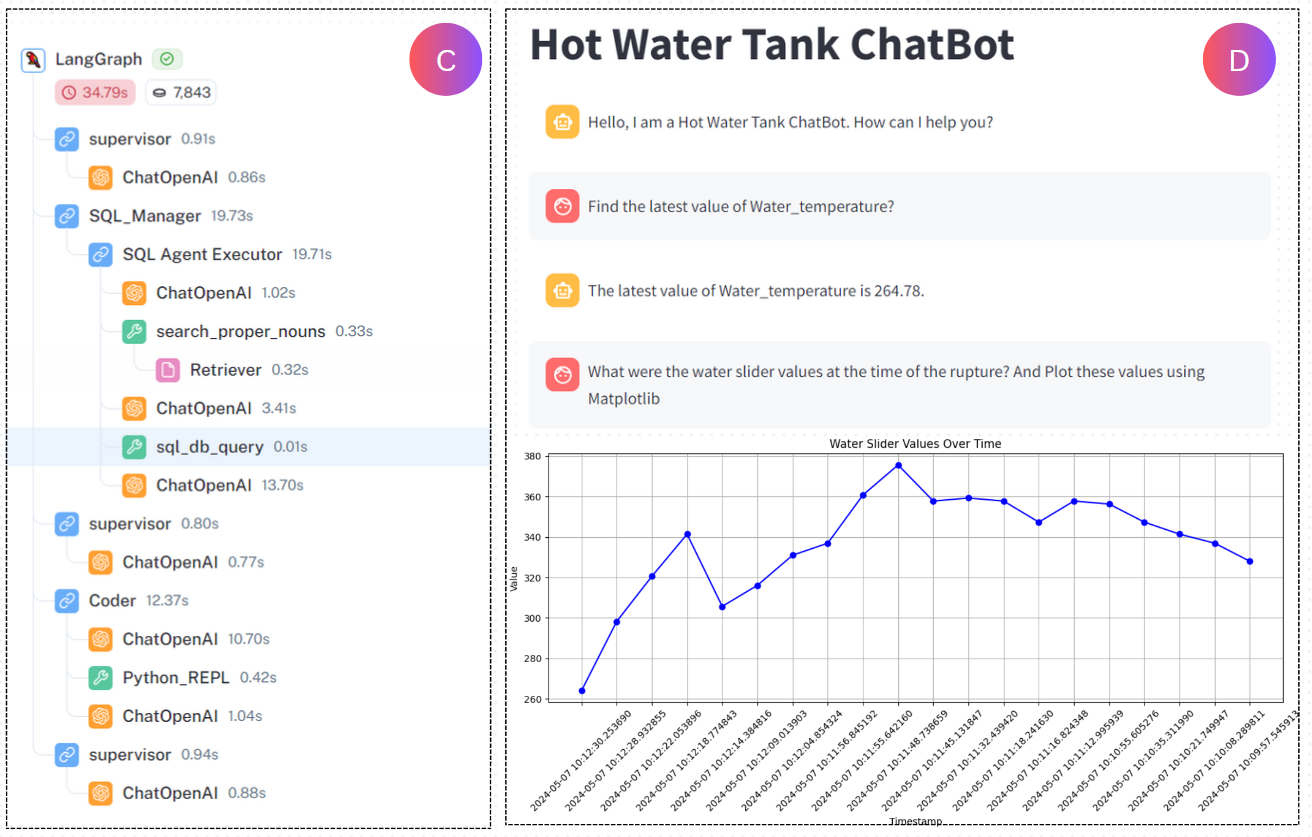
\includegraphics[width=.85\textwidth]{MX_Papers/Paper12/images/Result.PNG}
    \caption{Data analysis and visualization}
    \label{fig:results}
\end{figure*}


\subsection{LLM Agents integration}


Section \ref{sec:methodology} delineates the roles of various LLM agents, specifically the Info Agent with RAG, SQL Agent, and Python Coder, which are designed to facilitate intelligent analysis and visualization of IEC 61499 control systems. To accomplish this, LangGraph is employed to develop a stateful, multi-actor application. Illustrated in Figure \ref{fig:Architecture} (B), a collective of agents is organized, managed by an Agent Supervisor responsible for delegating tasks between agents. The programming for each agent node is streamlined through the use of the AgentExecutor class from LangChain, enhancing the system's efficiency.  The Agent Supervisor plays a pivotal role, not only managing the interactions among the agents but also utilizing function calling to select the subsequent worker node or terminate the processing. 

\begin{lstlisting} 
members = [ "Info_Agent", SQL_Manager", "Coder"]
system_prompt = (
    """
     You are a supervisor tasked with managing a conversation between the
     following agents:  {members}. Given the following user request,
     respond with the agents to act next. Each agent will perform a
     task and respond with their results and status. When finished,
     respond with FINISH.
     """
)
options = ["FINISH"] + members
prompt = ChatPromptTemplate.from_messages(
    [
        ("system", system_prompt),
        MessagesPlaceholder(variable_name="messages"),
        (
            "system",
            "Given the conversation above, who should act next?"
            " Or should we FINISH? Select one of: {options}",
        ),
    ]
).partial(options=str(options), members=", ".join(members))
supervisor_chain = (
    prompt
    | llm.bind_functions(functions=[function_def], function_call="route")
    | JsonOutputFunctionsParser()
\end{lstlisting}

The provided Python script demonstrates the implementation of a supervisory agent in a multi-agent system using a LLM. This agent oversees the coordination and execution of tasks by two specific agents, named "Info\_Agent","SQL\_Manager" and "Coder." The supervisory role is facilitated through a structured conversation flow, defined within a system prompt that instructs the supervisor on how to manage interactions with these agents based on user requests. The supervisor's decision-making process is aided by an interactive prompt template that integrates messages and options for routing the next action, either to continue with another agent or to conclude the process (FINISH).

A custom function, `route`, is defined to simplify the process of selecting the next agent to act. This function is part of the function calling capabilities provided by the LLM, which enhances the ease of output parsing and decision-making. The system is designed to iteratively consult the supervisor to determine the sequence of agent activation until the workflow is complete, ensuring all tasks are addressed in response to the user's initial request. This structure not only optimizes task distribution among agents but also maintains a clear and manageable workflow within the multi-agent system. The setup is now prepared to initiate the construction of the graph, following the steps laid out earlier for defining the state and worker nodes.

\begin{lstlisting} 
class AgentState(TypedDict):
    messages: Annotated[Sequence[BaseMessage], operator.add]
    next: str
sql_agent = create_sql_agent( llm=sql_llm, db=db, extra_tools=[retriever_tool], prompt=full_prompt, agent_type="openai-tools",verbose=False,)
sql_node = functools.partial(sql_agent_node, agent=sql_agent, name="SQL_Manager")
code_agent = create_agent(llm, [python_repl_tool], "You may generate safe python code to analyze data and generate charts using matplotlib.")
code_node = functools.partial(agent_node, agent=code_agent, name="Coder")
workflow = StateGraph(AgentState)
workflow.add_node("Info_Agent", info_node)
workflow.add_node("SQL_Manager", sql_node)
workflow.add_node("Coder", code_node)
workflow.add_node("supervisor", supervisor_chain)
for member in members:
    workflow.add_edge(member, "supervisor") 
conditional_map = {k: k for k in members}
conditional_map["FINISH"] = END
workflow.add_conditional_edges("supervisor", lambda x: x["next"], conditional_map)
workflow.set_entry_point("supervisor")
graph = workflow.compile()
\end{lstlisting}

This Python code snippet outlines the creation of a stateful, multi-actor workflow using a graph-based architecture designed for task delegation among Large Language Model (LLM) agents. The `AgentState` class, enriched with annotations to manage state updates, serves as the foundational state input for each node in the workflow graph. Specifically, SQL and code agents are instantiated with specified tools and prompts, and linked to corresponding graph nodes named "SQL\_Manager" and "Coder" respectively. The graph, defined as a `StateGraph`, integrates these nodes and establishes a supervisory node responsible for orchestrating the task flow and directing subsequent agent actions based on the conditionally mapped outcomes from each node. Edges are added to ensure that each agent node reports back to the supervisor upon completing its tasks, with the supervisor node determining the next course of action, whether routing to another node or concluding the process. The workflow is finalized by setting an entry point and compiling the graph, thus readying the system for operational execution.


\subsection{Dynamic AI Visualizer Data App}

In the recent experimental setup, a sophisticated multi-actor system employing large LLM agents was developed to interface with HMI (Figure \ref{fig:Architecture} (A3)) through REST APIs. Concurrently, a chatbot data visualizer was constructed to facilitate advanced data analysis and visualization through a web interface (Figure \ref{fig:results} (D)). This dual-interface system not only enhances in-factory operations but also supports remote access, thus broadening its applicability and utility. The Web application, pivotal for remote interactions, was developed using the Streamlit framework \cite{streamlit2023homepage}, which efficiently transforms data scripts into shareable web applications. While Streamlit was chosen for its specific capabilities, the experiment acknowledges that alternative web frameworks could also be utilized to construct the frontend architecture. This flexibility in technology selection underscores the adaptability of the system to various operational needs.



\section{Results}

The hot water tank experiment was carried out multiple times, during which data pertaining to 20 variables (Figure \ref{fig:Architecture} (B2)) were systematically recorded in various tables within a PostgreSQL database. This experiment utilized an IEC 61499 application to manufacture both product1 and additional product recipes, adhering to specified recipe sequences. The vast database, in scope, contained approximately 100,000 entries distributed in different tables. The tank experienced numerous ruptures throughout the experiment, all of which were subsequently repaired and documented. With the comprehensive data collection phase completed, the focus has now shifted to data analysis. Numerous queries have been formulated and are currently being represented in tabular format for detailed examination.

\begin{table*}
\centering
\resizebox{\textwidth}{!}{
\begin{tabular}{|>{\raggedright\arraybackslash}m{5cm}|>{\raggedright\arraybackslash}m{3cm}|>{\raggedright\arraybackslash}m{5cm}|>{\raggedright\arraybackslash}m{3cm}|}
\hline
\textbf{User Input} & \textbf{Agents} & \textbf{Output} & \textbf{Time in Seconds} \\ \hline
What conditions lead to a tank rupture? & Q\&A Agent & A tank rupture occurs when the water level exceeds 350.00 & 07.62 \\ \hline
Find the latest value of ECC STATE? & SQL Agent & The latest value of ECC STATE is "Wait", and the timestamp at which this action occurred is 2024-05-07 10:12:33.865736 & 10.20 \\ \hline
When did the tank last rupture? & SQL Agent & The tank last ruptured on May 7, 2024, at 10:12:31. & 8.38  
\\ \hline How long did it take to fix the tank? & SQL Agent & It took 1 minute and 9 seconds to fix the tank & 18.48 \\ \hline
What were the values of the water slider at the time of the rupture? And plot these values using Matplotlib. & SQL Agent, Coder Agent, & The graph displaying the Water Slider Values over time has been plotted using the provided data. You can view the graph in Figure \ref{fig:results} (D). Each point represents a Water Slider Value at a specific timestamp. & 34.79 \\ \hline 
\end{tabular}
}
\vspace{2mm} % 
\caption{Query responses and timings}
\end{table*}


The experiment used gpt-3.5-turbo as the primary LLM, although integration with various open-source models was noted to be feasible. 
The involvement of agents in each query is detailed in Table 1. The details of the execution of the final query, facilitated by LangGraph, are depicted in Figure \ref{fig:results} (C). This illustrates the execution process and the time that each agent takes to complete their respective tasks. It was observed that the complexity of the queries significantly affects the execution time. Specifically, as the complexity of the queries increases, or as more agents are involved in the processing, the time required to reach a conclusion increases. Consequently, for complex analytical tasks, the time to obtain a final answer might exceed 30 seconds, depending predominantly on the capabilities of the model and the intricacy of the queries posed. 



\section{Conclusion and future work}
\label{sec:conclusion}

This paper presented a multi-actor system integrating LLMs with IEC 61499-based control systems for intelligent analysis and visualization. Using advanced frameworks such as LangChain and LangGraph, the system significantly enhances the accessibility and usability of ICS through natural language interactions. The employment of LLMs in various roles—from SQL query generation to complex data analysis and predictive maintenance—illustrates the versatility and efficacy of conversational AI in streamlining operations and improving decision-making processes within industrial settings. The case study on the Hot Water Tank IEC 61499 application highlighted the practical application of this system, effectively managing complex queries and operations, facilitating efficient data handling, and bridging the gap between complex industrial data and actionable insights.

In the future, the system will be expanded to include integration with other open-source models to broaden capabilities and adaptability, especially in real-time processing improvements for faster decision making. Enhancements in predictive analytics will focus on foreseeing potential issues through advanced machine learning algorithms, improving preventive maintenance strategies. In addition, efforts will be made to broaden the range of applications to diverse industrial environments, improve security measures and privacy protocols, and refine the human-machine interface. These developments aim to make ICS more adaptive, robust, and user-friendly, catering to evolving industrial needs and technological advances.


\section{Acknowledgements}
This research was supported in part by the Horizon Europe Zero-SWARM project funded by the European Commission (grant agreement: 101057083).

%%% Put references here
\putbib
\end{bibunit} 